\documentclass[12pt,twocolumn,a4paper,oneside]{article}

\usepackage{silence}
% check out persiantex/bidi#20
\WarningFilter{biditools}{Patching `\enddocument' failed}

\usepackage{hyperref}

\usepackage{graphicx}
\graphicspath{{img}}

\newcommand{\titlefa}{%
طراحی کنترل‌کننده سیستم نورپردازی پیکسلی \lr{RGB} مبتنی بر برنامه کاربردی وب با رویکرد اینترنت اشیاء}

\newcommand{\authorfa}{محمدامین صامتی}

\newcommand{\rawsupervisorfa}{حامد خوش‌نیت}
\newcommand{\supervisorfa}{دکتر\space\rawsupervisorfa}

\newcommand{\departfa}{دانشکده مهندسی برق و کامپیوتر}

\newcommand{\instfa}{دانشگاه صنعتی اراک}

\newcommand{\datefa}{شهریور ۱۴۰۰}

\newcommand{\titleen}{Design of RGB Pixel System Controller based on Web Application with IoT Approach}

\newcommand{\authoren}{Mohammad Amin Sameti}

\newcommand{\supervisoren}{Dr. Hamed Khoshniyat}

\newcommand{\insten}{Arak University of Technology}

\newcommand{\dateen}{September 2021}


\usepackage{geometry}
\geometry{left=14mm, right=14mm, top=10mm, bottom=14mm}

\usepackage{titlesec}
\titleformat{\section}{\normalsize\bfseries}{\thesection}{.5em}{}
\titleformat{\subsection}{\normalsize\bfseries}{\thesubsection}{.5em}{}
\titleformat{\subsubsection}{\bfseries}{\thesubsubsection}{.5em}{}
\titlespacing{\section}{10pt}{2.5ex}{0pt}
\titlespacing{\subsection}{0pt}{2ex}{0pt}

\usepackage{xepersian}

\settextfont{Nazli}
\setlatintextfont{Liberation Serif}

\title{\vspace{-8mm}{\centering\titlefa\par}\lr\titleen}

\newcommand{\makeauthor}[3]{{#1}\\
  {\normalsize\departfa, \instfa}\\
  \lr{#2}\\
  شماره تلفن: {#3}}

\author{%
  \makeauthor{\authorfa}{mamins1376@gmail.com}{۰۹۳۹۴۴۵۳۳۴۷}\and%
  \makeauthor{\rawsupervisorfa}{hkhoshniyat@arakut.ac.ir}{۰۸۶۳۳۴۰۰۶۱۴}}

\date{}

\begin{document}

\twocolumn[{%
  
\includegraphics[width=\textwidth]{header}%
  \let\newpage\relax\maketitle}]%

{\bfseries{چکیده-}}
سیستم‌های نورپردازی سه رنگ آدرس‌پذیر\LTRfootnote{Addressable RGB LED Lighting System} قابلیت کنترل از راه دور را به صورت پویا دارند و با امکانات مختلفی در بازار موجود هستند. این سیستم‌ها متشکل از ۴ بخش اصلی هستند که هرکدام کارکرد خاص خود را داشته و قابلیت‌های متفاوتی نیز دارند. برای ارتباط کاربر با کنترلر در این سیستم، از پروتکل‌های بی‌سیم استفاده می‌شود که مزایا و معایبی دارند. نویسندگان نمونه‌ی از این سیستم ساخته‌اند که تمرکز آن روی کاهش هزینه و بهبود جلوه‌های هماهنگ با صوت و موسیقی است و برای طراحان صحنه‌های هنری و ورزشی بستر جدیدی برای خلاقیت و نوآوری فراهم می‌سازد. 

ریسه‌های قابل آدرس‌دهی پیکسلی پروتکل خاص خود را داشته که توانایی ایجاد ریسه‌های بلند و برنامه‌پذیر با سرعت مناسب را ممکن می‌کند. این  ریسه‌ها قابل استفاده در محیط بسته و باز هستند و در صورتی که منبع تغذیه با توان کافی استفاده شود می‌توان با کنترلر ساخته شده برنامه‌های جذابی را در محیط‌های کوچک یا گسترده طراحی نمود و به صورت زنده از طریق رایانه یا تلفن همراه هوشمند آن را به اجرا گذاشت.

کاربر پس از اتصال به کنترلر و راه‌اندازی آن، از برنامه‌کاربردی مبتنی بر وب استفاده می‌کند و یا برای دسترسی به تمام قابلیت‌های موجود، من جمله نورپردازی خودکار با صدای پخش شده توسط تلفن هوشمند خود و بازپخش برنامه‌های نورپردازی قبلی، برنامه‌ی مخصوص دستگاه خود را دریافت و نصب می‌کند و بدین طریق نمایش دلخواه خود را بدون نیاز به دسترسی فیزیکی به سیستم نورپردازی و از راه دور--چه از شبکه داخلی محل نمایش و چه از طریق شبکه جهانی اینترنت--پخش و کنترل می‌کند.

{\bfseries{کلید واژه-}}
اینترنت اشیاء، نورپردازی،
\lr{LED} پیکسلی، 
\lr{RGB}،
برنامه کاربردی وب، کنترلر،
\lr{ESP8266}

\begin{latin}
{\bfseries Abstract-}
Addressable RGB LED Lighting Systems can be controller remotely to achieve dynamic effects, and are accessible in the market with a variety of features. In order to make a connection between the user and controller, different wireless communication protocols are available which have their own strengths and weaknesses. The authors have made a prototype of such system focusing on cost reduction and enhancing audio-synchronizsed effects which will bring a new platform for artistic and martial arts' scene designers to innovate and create dynamic and reactive performances.

Addressable Pixel strips have their own set of protocols which makes making long, controllable and responsible cascaded chain of strips possible. Such strips can be used in indoor or open places which, combined with a powerful enough power supply, can empower the designer or user to make amazing scenes in small or wide areas with the help of their computer or smartphone.

After the connection has been established and initial setup is completed, the user will use the Web-based application or, in order to be able to use all the available features including the ability to use his/her device's system audio as a source for automatic light show effect generation or replaying previously-recorded program, install the native application for their corresponding mobile platform. Thus the user can play and control their favorite program regardless of where they actually are--whether connected directly to their local network or connected through the Internet from a remote location.

{\bfseries Keywords-} Internet of Things, IoT, Lighting system, Pixel LED, Addressable RGB strip, Web Application, ESP8266
\end{latin}

\section{مقدمه}
در دهه‌ی اخیر بازار خاصی برای سیستم‌های نورپردازی و روشنایی خانگی مبتنی بر دیودهای نوری ایجاد شده است. این سیستم‌ها توانایی تنظیم رنگ را به صورت زنده یا از پیش برنامه‌ریزی شده دارند و اغلب رابطی برای کنترل از راه دور، از طریق ارتباط مادون قرمز و یا امواج رادیویی در آن‌ها تعبیه گردیده است.

\subsection{نحوه کار}

کاربر با تلفن‌هوشمند، رایانه‌لوحی و یا رایانه شخصی یا قابل حمل خود به کنترلر یا نقطه دسترسی وای‌فای متصل می‌شود؛ گرچه لزومی به وجود دستگاه اخیر نیست زیرا کنترلر نیز می‌تواند خود به عنوان یک نقطه دسترسی مستقل عمل کند. پس از اعمال تنظیمات مربوطه و ارائه‌ی مشخصات دیودهای وصل شده، کاربر می‌تواند نور دلخواه خود را تنظیم کند.

بلوک‌های تشکیل‌دهنده‌ی سیستم در شکل
\ref{fig:diagram}
دیده می‌شود. این سیستم‌ها از چهار قسمت کنترل از راه دور، خروجی نوری، منبع تغذیه و کنترلر یا راه‌انداز تشکیل شده‌اند؛ که امکان ادغام دو یا سه مورد آخر به عنوان یک واحد مستقل وجود دارد. خروجی نوری ممکن است فقط یک دیود نوری چند رنگ باشد یا آرایه‌ای از دیودهای مجزا یا بلوک‌های تک‌رنگ باشد. به همین صورت کنترلرها ممکن است تک‌رنگ باشند یا توانایی اختصاص رنگ به هر دیود یا گروه دیودها را داشته باشد. دیودهایی که به صورت گروهی متصل شده‌اند ممکن است سری یا موازی باشند که این انتخاب تعیین کننده‌ی ولتاژ تغذیه مورد نیاز برای راه‌اندازی آنهاست. همچنین تعداد دیودها مشخص‌کننده‌ی جریان و طبعا توان مصرفی است که توقع می‌رود منبع تغذیه قادر به تأمین آن باشد.

\begin{figure}[ht]
\centering
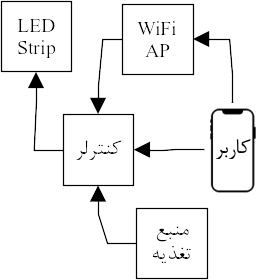
\includegraphics[scale=0.6]{diagram}
\caption{بلوک دیاگرام سیستم}
\label{fig:diagram}
\end{figure}

\subsection{دیودهای نوری آدرس‌پذیر}
دیودهای نوری آدرس‌پذیر، توان دریافتی از منبع تغذیه را به در خواست کنترلر به نور تبدیل می‌کنند؛ که آدرس‌پذیر بودن آن‌ها نشانگر توانایی نشان‌دادن چندین رنگ مختلف در آن واحد است. هر دیود یا گروه دیودها به یک مدار مجتمع مخصوص متصل است که با کنترل جریان مربوط به هر رنگ، طیف رنگ و میزان روشنایی را طبق فرمان کنترلر تعیین می‌کند.

\subsubsection{مدار مجتمع \lr{WS2811}}
همان‌طور که گفته شد، خروجی نوری سیستم متشکل از دیودهای نوری است. این دیودها در تعداد بالا (معمولا  ۵۰ یا ۱۰۰ دیود سه رنگ در هر ریسه) موجود بوده و ریسه‌ها قابلیت اتصال آبشاری به یکدیگر را دارند. ولتاژ تغذیه آن‌ها ۵ یا ۱۲ ولت است که بستگی به تکی یا گروهی بودن هر گروه همرنگ دارد. به دلیل تعداد به نسبت بالای دیودها نیاز است تا روشی برای فرمان‌پذیری از کنترلر به کار گرفته شود تا علاوه بر استفاده از سیم‌های ورودی کمتر، سرعت بالایی را برای نمایش و به روزرسانی رنگ هر دیود فراهم نماید. در ریسه‌های مبتنی بر مدار مجتمع \lr{WS2811}، ارتباط از طریق استفاده از یک سیم داده‌ی غیرهمزمان تحقق می‌پذیرد که پروتکل مخصوص خود را برای انتخاب رنگ دارد. این مدار مجتمع توانایی انتخاب یک رنگ برای یک دیود و یا گروهی از دیودهای به هم متصل را دارد (شکل  \ref{fig:ws2811-wiring}).

از منظر الکتریکی، این قطعه یک منبع جریان سه کانال است که طبق پروتکل مخصوص خود، میزان جریان عبوری از هر کانال قرمز، سبز یا آبی را با دقت ۸ بیت تنظیم می‌کند. برای اتصال چند دیود به یک مدار مجتمع و تشکیل گروه‌های همرنگ، دیودهای با رنگ‌های یکسان با هم سری شده و جریان یکسانی از آن‌ها عبور می‌کند.

پروتکل مورد استفاده، یک سیگنال دیجیتال ۲۴ بیتی مدوله شده با پهنای پالس است که در آن همه‌ی بیت‌های مربوط به گروه از دیودها به یکباره فرستاده می‌شوند، پس از مدت زمان معینی سیگنال گروه دوم ارسال می‌شود و همین روند تا ارسال رنگ برای آخرین گروه تکرار می‌شود. پایه خروجی مدارات مجتمع هر گروه به صورت متوالی به ورودی گروه قبلی وصل می‌شود و ورودی اولین گروه از کنترلر دریافت می‌گردد. هر آی‌سی اولین گروه ۲۴ بیتی از داده‌ها را دریافت می‌کند و بقیه‌ی بیت‌ها را دست نخورده به آی‌سی بعدی منتقل می‌سازد. بدین ترتیب، از لحاظ نظری می‌توان یک توالی بی‌نهایت طولانی از گروه‌های دیودی ایجاد کرد.

\begin{figure}[ht]
\centering
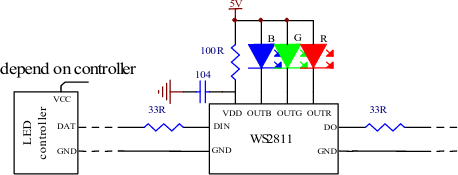
\includegraphics[width=\linewidth]{ws2811-wiring}
\caption{اتصالات الکتریکی مدار مجتمع \lr{WS2811}\cite{ws2811:datasheet}}
\label{fig:ws2811-wiring}
\end{figure}

البته این روش معایب خود را نیز دارد؛ از جمله محدودیت در سرعت تغییر رنگ کل ریسه که منجر به کاهش سرعت قابل ملاحظه‌ای در ریسه‌های بسیار بلند خواهد شد. علت این امر این است که هر مدار مجتمع تا وقتی اطلاعات رنگ مربوط به خود را دریافت نکند اقدام به باز ارسال بقیه اطلاعات نخواهد کرد و در نتیجه برای به‌روز رسانی هر گروه لازم است دوباره رنگ گروه‌های قبل از آن مجددا فرستاده شود. این محدودیت موجب می‌شود به‌روزرسانی یک به یک گروه‌های دور از ابتدای ریسه از لحاظ زمانی به صرفه نباشد و کندی قابل توجهی در نمایش نهایی ایجاد کند؛ پس بهتر است رنگ هر گروه ابتدا در حافظه‌ای ذخیره شود و در بازه‌های زمانی مشخصی کل ریسه به روز رسانی شود.

\subsection{کنترلرهای موجود}
کنترلرهای موجود اغلب سازگار با یکی از پروتکل‌های
\lr{Bluetooth}، \lr{Wi-Fi}،
کنترل از راه دور مادون قرمز، فرستنده‌ی رادیویی مخصوص و یا ترکیبی از این موارد هستند. کنترل مادون قرمز به علت سادگی فقط توانایی تخصیص یک رنگ به کلیه دیودها را دارد در حالی که در صورت استفاده از دیگر رابط‌ها امکان کنترل پیشرفته‌تر نیز وجود دارد؛ از جمله تعیین رنگ گروهی، تعیین رنگ‌های متغییر با زمان به صورت از پیش برنامه‌ریزی شده یا زنده (که می‌تواند به صورت دستی یا پاسخگو به شرایط نور محیطی و یا تصویر ثابت باشد).

کنترلرهایی که مجهز به فناوری \lr{Wi-Fi} هستند ذاتاً مبتنی بر شبکه‌ی پروتکل اینترنت بوده و امکان کنترل از راه دور و بر بستر اینترنت را دارند؛ که البته ارتباط زنده و همزمان کنترل و کنترلر نیازمند تأخیر پایین شبکه و دسترسی به پهنای‌باند مناسب است. بدین ترتیب، مفهوم اینترنت اشیاء برای چنین سیستم‌هایی معنا پیدا می‌کند.

در ادامه چندین نمونه‌ی رایج از این کنترلرها با قابلیت‌های متفاوت را مختصراً بررسی می‌کنیم.

\subsubsection{کنترلرهای مبتنی بر بلوتوث}
بلوتوث\LTRfootnote{Bluetooth} یک استاندارد کوتاه-برد بی‌سیم است که برای تبادل داده میان ابزارهای ثابت یا متحرک در باند فرکانسی فرابالا
\lr{(UHF\LTRfootnote{Ultra High Frequency})}
در محدوده‌ی ۲٫۴ تا ۲٫۴۸ گیگاهرتز استفاده می‌شود\cite{bluetooth-freq}. دستگاه‌های مبتنی بر این استاندارد در حالت رایج خود به توان ارسالی ۲٫۵ میلی‌وات محدود هستند که بردی حدود ۱۰ متر را برای کانال مخابراتی تعیین می‌نماید\cite{bluetooth-range}.

یک نمونه از این کنترلر، علاوه بر اتصال با روش بلوتوث به کنترل، می‌تواند از طریق یک ترمینال تعبیه شده با رایانه‌ی بالادستی و با پروتکل سریال ارتباط برقرار کند\cite{patent:CN103987158A}.

\subsubsection{کنترلرهای مبتنی بر وای‌فای}

\begin{figure}[ht]
\centering
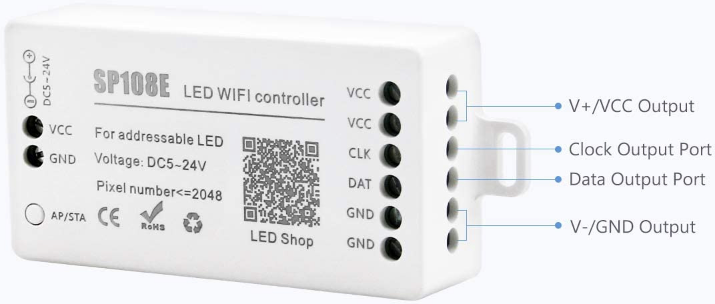
\includegraphics[width=\linewidth]{controller}
\caption{یک نمونه کنترلر مبتنی بر \lr{Wi-Fi}\cite{amzn:B07DDB6JHJ}}
\label{fig:controller}
\end{figure}

وای‌فای\LTRfootnote{Wi-Fi} یک خانواده از پروتکل‌های شبکه‌ی بی‌سیم است که عموماً برای شبکه‌های محلی و دسترسی به اینترنت استفاده می‌شود. همانند استاندارد بلوتوث، این پروتکل نیز بر باند فرکانسی ۲٫۴ گیگاهرتز مبتنی است؛ گرچه در نسخه‌های جدیدتر این استاندارد توانایی بهره‌گیری از باند ابربالا
\lr{(SHF\LTRfootnote{Super High Frequency})}،
در محدوده فرکانسی ۵ گیگاهرتز نیز در نظر گرفته شده است. از دید ساختار شبکه در مدل
\lr{(OSI\LTRfootnote{Open Systems Interconnection})}،
این پروتکل، پایین‌ترین دو لایه (لایه‌ی فیزیکی و لایه‌ی پیوند داده) را شامل می‌شود و می‌تواند از داده‌های تبادل شده در لایه‌های مذکور در برابر تغییرات نا‌خواسته بر اثر نویز محیطی و یا دستکاری عامدانه‌ی اطلاعات و یا شنود آنها توسط فرد سومی که به کانال بی‌سیم دسترسی دارد جلوگیری کند؛ اما نسخه‌های قدیمی‌تر این استاندارد روش‌هایی را برای رمزنگاری داده‌ها معرفی می‌کند که بعداً مشخص شد امنیت اطلاعات را تضمین نمی‌کنند و در حال حاضر منسوخ محسوب می‌گردند (به طور خاص
\lr{WEP\LTRfootnote{Wired Equivalent Privacy}}
و
\lr{WPS\LTRfootnote{Wi-Fi Protected Setup}}).
روش‌های جدیدتری به این منظور ارائه گردیده اند که از امنیت بسیار بهتری برخوردار هستند\cite{wi-fi}.

\begin{figure}[ht]
\centering
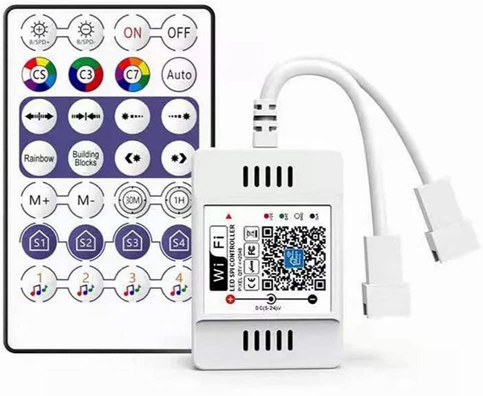
\includegraphics[width=\linewidth]{controller2}
\caption{یک نمونه کنترلر تجاری مبتنی بر \lr{Wi-Fi}, \lr{Bluetooth} و نور مادون قرمز\cite{amzn:B09BMBHDWN}. در سمت راست کنترلر و در سمت چپ کنترل از راه دور مادون قرمز مشاهده می‌شود.}
\label{fig:controller2}
\end{figure}

به علت برد بیشتر اتصال‌های مبتنی بر این استاندارد (حدود ۲۰ متر برای نقطه‌های دسترسی داخلی و بعضاً تا ۱۵۰ متر برای بعضی از مدل‌های مناسب برای فضای باز\cite{wi-fi}) از مزیت‌های کنترلرهای استفاده کننده از وای‌فای می‌توان به برد بیشتر آنها و قابلیت استفاده از آنها به صورت نسبتاً پراکنده و در مناطق وسیع اشاره کرد. همچنین بر خلاف استاندارد بلوتوث، امکان عمل‌کردن واحدها به صورت تکرار کننده\LTRfootnote{Wi-Fi Repeater}‌ نیز در این استاندارد گنجانده شده است و شرایط لازم برای ایجاد آرایه‌های بلندی از ابزارهای متصل به هم که یک شبکه‌ی مشترک را در دسترس قرار می‌دهند فراهم می‌سازد. به عنوان مثال، کنترلرهایی وجود دارد که به منظور استفاده‌ی خارجی تهیه شده و ضد آب بودن، منعطف بودن و تحمل محدوده دمایی مناسب برای آن در نظر گرفته شده است\cite{patent:CN210485639U}\cite{patent:CN212156755U}\cite{patent:CN209213534U}.

معمولاً به علت تنوع پروتکل‌های مورد استفاده برای برقراری ارتباط میان کنترلر و ریسه‌ی دیودها، کنترلرهای تجاری جهت افزایش سازگاری محصول پروتکل‌های فراوانی را پشتیبانی می‌کنند. پروتکل‌های دیودها از یک سیم (نوع غیرهمزمان) یا نهایتا دو سیم (نوع همزمان) برای داده استفاده می‌کنند و به همین علت، هزینه‌های سخت‌افزاری چندانی نخواهد داشت و قسمت الکتریکی پروتکل به سادگی با دو خروجی تحقق پذیر است. یک نوع کنترلر که از ۱۳ نوع خروجی پشتیبانی می‌کند در شکل \ref{fig:controller} نشان داده شده است\cite{amzn:B07DDB6JHJ}.

\section{سیستم نورپردازی ساخته شده}

\begin{figure}[ht]
\centering
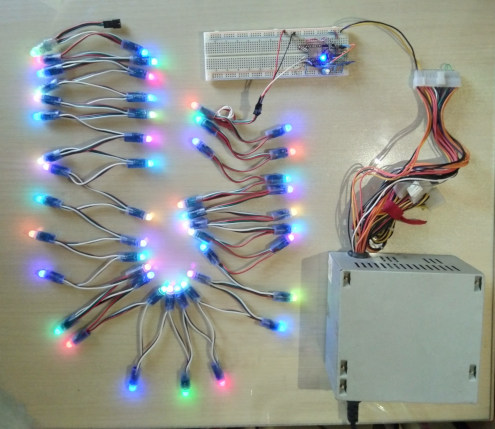
\includegraphics[width=\linewidth]{setup}
\caption{سیستم ساخته شده}
\label{fig:setup}
\end{figure}

سیستم ساخته شده‌ در شکل \ref{fig:setup} مشاهده می‌شود. جعبه‌ی سمت راست تصویر یک منبع تغذیه‌ی ۵ ولتی را نشان می‌دهد که توانایی لازم برای تهیه توان مصرفی دستگاه را دارد. در سمت چپ تصویر ریسه‌ی دیودها دیده می‌شود و شامل ۵۰ دیود ۳ رنگ کنترل شونده با پروتکل \lr{WS2811} است. بردی که این دو قسمت را به یکدیگر مرتبط می‌کند حاوی یک ماژول وای‌فای با مدار مجتمع \lr{ESP8266}‌ است که یک پردازنده مبتنی بر معماری \lr{Xtensa} بوده و ادوات لازم برای برقراری ارتباط با نقطه‌ی دسترسی وای‌فای یا ایجاد آن برای کاربر را دارد\cite{esp8266}.

\begin{figure}[ht]
\centering
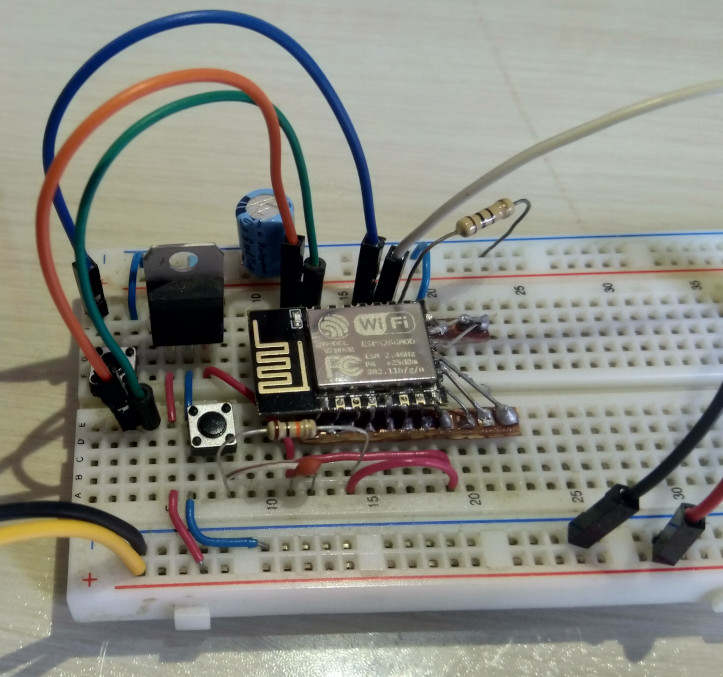
\includegraphics[width=\linewidth]{close-up}
\caption{نمای نزدیک از کنترلر}
\label{fig:close-up}
\end{figure}

در شکل \ref{fig:close-up} نمای کنترلر ساخته شده از نزدیک دیده می‌شود. در وسط تصویر ماژول وای‌فای قابل برنامه‌ریزی مشاهده می‌شود که سیم سفید خروجی آن بوده و به ریسه متصل می‌گردد. دو سیم مشکی و زرد پایین تصویر ورودی ۵ ولت است که برای تغذیه‌ی ریسه و ماژول کاربرد دارد، گرچه این ماژول نیاز به ولتاژ ۳٫۳ ولت دارد و مدار مجتمع سمت چپ تصویر که یک مبدل ولتاژ خطی است این تبدیل را انجام می‌دهد. دو کلید واقع در سمت چپ برای شروع مجدد برنامه و فعال کردن حالت برنامه‌ریزی استفاده می‌شوند.

\subsection{راه‌اندازی}
اولین باری که کنترلر روشن می‌شود، نقطه دسترسی را برای اتصال مستقیم کنترل کاربر فراهم می‌کند. در صورت تمایل کاربر می‌تواند مشخصات نقطه دسترسی دیگری را (که می‌تواند یک مسیریاب شبکه یا کنترلر دیگری هم باشد) وارد کند تا اتصال بین کاربر و کنترلر بر آن بستر باشد.

مزیت اتصال به نقطه دسترسی مجزا در فراهم آوردن امکان اتصال همزمان یک کاربر به چندین کنترلر است که می‌تواند موجب گسترش محدوده‌ی پوشش خروجی‌ها، توزیع بهینه‌تر مصرف توان (استفاده از چندین منبع تغذیه کم توان‌تر به جای یک منبع پرتوان)، بیشتر کردن برد شبکه و در نتیجه عدم نیاز به نقطه دسترسی بلند-برد شود.

پس از راه‌اندازی بستر شبکه، کاربر یک از دو برنامه کاربردی مربوط به کنترلر را استفاده می‌کند. برنامه اول یک برنامه تحت وب است که نیازی به نصب نداشته و مستقیماً از هر مرورگر وب به‌روزی قابل استفاده است، گرچه امکانات تعبیه‌شده در آن به نسبت برنامه‌ی دوم کمتر است. شمایی از این برنامه در شکل \ref{fig:wled}‌ مشاهده می‌شود. در این صفحه به کمک دایره‌ی مرکزی می‌توان رنگ دیودها را تنظیم کرد و یا رنگ‌های از پیش انتخاب شده‌ای را فعال کرد.

\begin{figure}[ht]
\centering
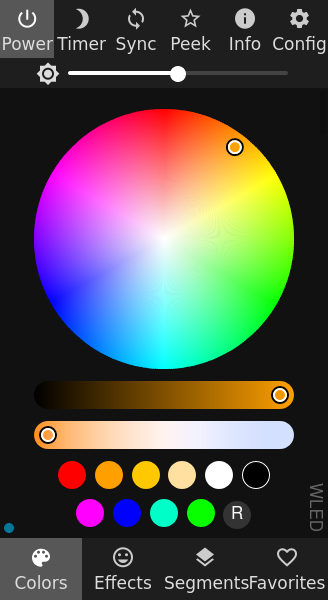
\includegraphics[scale=0.5]{wled}
\caption{برنامه‌ی مبتنی بر وب}
\label{fig:wled}
\end{figure}

برنامه دوم مخصوص سیستم‌عامل کاربر بوده و پس از نصب قابل استفاده است. چون در حال حاضر سیستم‌عامل‌ها به برنامه‌ی بومی خود اختیارات بسیار بیشتری نسبت به برنامه‌های تحت وب ارائه می‌دهند، طبیعتاً محدودیت‌های حاضر در پلتفرم وب رفع شده و امکان دسترسی به فضای بیشتر، تعامل با دیگر برنامه‌ها (برای اشتراک گذاری نورپردازی طراحی شده)، استفاده‌ی مستقیم از صدای پخش شده توسط سیستم‌عامل و بهره‌گرفتن از آن به عنوان منبع صدا (که برای ایجاد خودکار نورپردازی‌های مختلف و زنده کاربرد دارد) فراهم می‌گردد. بدین صورت کاربر می‌تواند برای هماهنگی نورپردازی با موسیقی، پس از راه‌اندازی اولیه‌ي برنامه‌ی مخصوص سیستم‌عامل از برنامه‌ی دلخواه خود برای پخش صدا استفاده کند؛ چه موسیقی، چه فیلم و چه هر رسانه‌ی دیگری (شکل \ref{fig:ledfx}).

برای هماهنگ‌سازی نورپردازی با موسیقی و ایجاد جلوه‌های جذاب بصری می‌توان از دو روش به تنهایی و یا به صورت ترکیبی استفاده نمود. در روش دستی، نوع مختلف جلوه‌ها توسط تدوین‌گر و با نرم‌افزار مخصوص طراحی و آماده می‌شود. از مزایای این روش می‌توان به انعطاف و اختیار تام در انتخاب جلوه‌ها و زمان‌بندی آن‌ها، و همچنین استفاده‌ی مجدد از جلوه‌ها، و نیاز به توان پردازشی بسیار کم اشاره کرد؛ اما از معایب این روش وقت‌بر بودن و نیاز به نیروی انسانی جهت برنامه‌ریزی است.

روش دیگر، استخراج اطلاعات لازم از موسیقی و ایجاد یک فضای چند بعدی از پارامترهای لحظه‌ای مربوطه (مانند بلندی صدا، طنین صدا و یا استخراج صدای خواننده یا یک ساز خاص) و سپس نگاشت آن‌ها به ابعاد مختلف جلوه‌های نوری روشنایی، رنگ یا سرعت پخش جلوه و در نهایت انتخاب از میان جلوه‌ها و پخش نتایج در خروجی است؛ چه به صورت لحظه‌ای و در زمان واقعی و چه به صورت از پیش پردازش شده. خوبی این روش در خودکار بودن آن است و پس از طراحی الگوریتم جلوه، دیگر نیازی به تدوین‌گر نیست. البته در صورتی که اجرای الگوریتم در زمان واقعی باشد نیاز به پردازنده‌ی مناسب با سرعت لازم وجود دارد. نمونه‌ای از چنین کنترلری وجود دارد که به کاربر امکان می‌دهد حالت دلخواه خود را از میان تعداد از پیش برنامه‌ریزی شده انتخاب کند\cite{amzn:B0792T73VB}. همچنین، مدل دیگری که امکان برنامه‌ریزی جلوه‌های دلخواه بصری را به کاربر ارائه می‌دهد نیز در دسترس است\cite{amzn:B01M4IX5FF}.

\begin{figure}[ht]
\centering
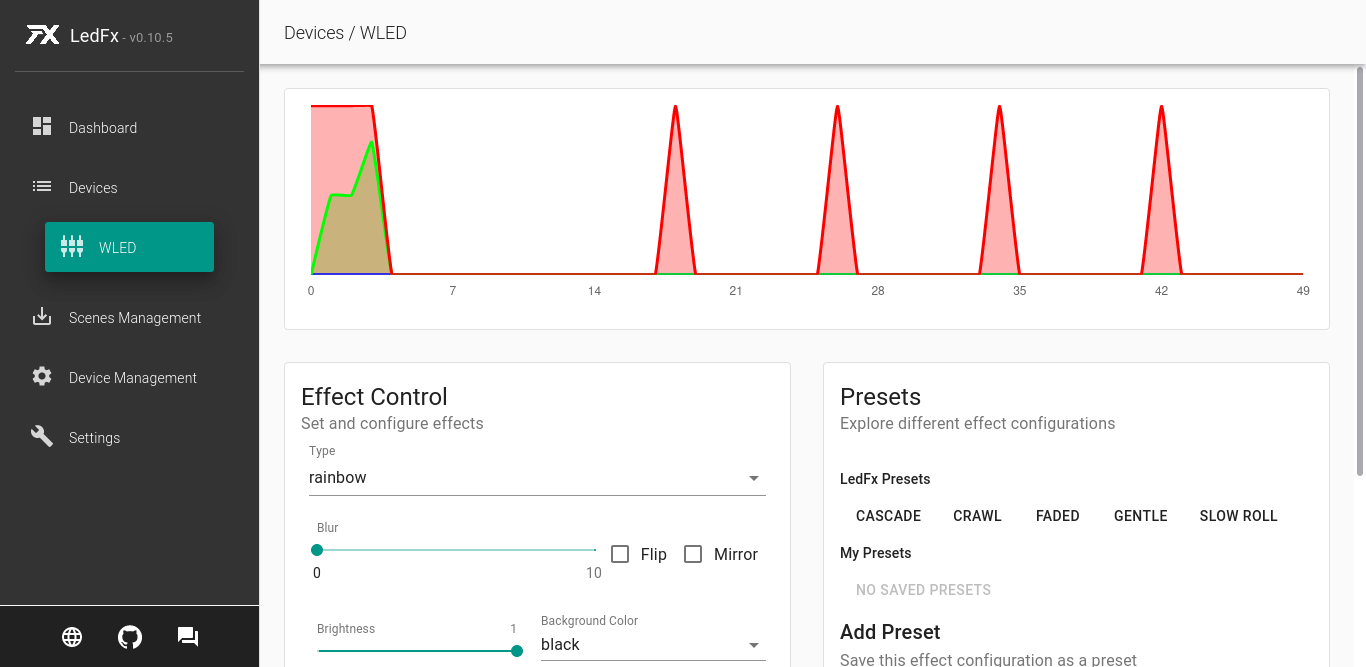
\includegraphics[width=\linewidth]{ledfx}
\caption{رابط برنامه‌ی بومی قابل نصب بر رایانه}
\label{fig:ledfx}
\end{figure}

\subsection{نوآوری‌ها}
در سیستم ارائه شده، امکان هماهنگ کردن خودکار نورپردازی با موسیقی زنده وجود دارد. همچنین امکان برنامه‌ریزی و اصلاح برنامه و ضبط و پخش مجدد نورپردازی نیز ممکن است. برنامه‌ی ضبط شده روی دستگاه کنترل کاربر ذخیره شده و امکان به اشتراک گذاری آن فراهم می‌گردد.

همچنین به منظور کاهش هزینه‌های تولید برای هر ابزار، کاهش فضای مورد استفاده و افزایش بهینگی مصرف توان، تمام نرم‌افزار مورد نیاز بر روی پردازنده‌ی مجهز به ادوات وای‌فای اجرا می‌شود و مستقیماً از طریق خروجی‌های مدار مجتمع حاوی پردازنده با ریسه‌ی دیودهای نوری ارتباط برقرار می‌کند.

\section{جمع‌بندی و نتیجه‌گیری}

طراحی سیستم‌های نورپردازی پیشرفته بیش از پیش در دسترس عموم قرار گرفته است و میان کاربران خانگی نیز جای خود را پیدا کرده است. طراحان فضای داخلی منازل مسکونی می‌توانند با استفاده‌ی مناسب از این ابزار جلوه‌ی جدیدی به ظاهر کار خود بدهند و پویایی دلخواه خود را در آن ایجاد کنند؛ مانند نور محیطی ثابت و یا نورپردازی داخلی مناسب پخش موسیقی یا فیلم و یا مناسبت‌ها و مراسم خاص. همچنین، با نوآوری‌های انجام شده و به وجود آمدن امکان هماهنگ‌سازی با اجرای هنرمندان و تدوین برنامه‌ی نورپردازی، طراحان صحنه نیز به این ابزار به راحتی دسترسی خواهند داشت و در اجراهای هنری (مانند تئاتر و سینما و کنسرت‌های موسیقی) و اجراهای ورزشی (مانند ورزش‌های نمایشی گروهی و برنامه‌های تلوزیونی) می‌توانند به عمق و کیفیت برنامه‌ی خود بیافزایند.

\bibliographystyle{ieeetr-fa}
\bibliography{references}

\end{document}
